\chapter{Post installation}
\label{chapter:post_install}

\section{Configure the administrator user}
Navigate your browser to \textit{http://localhost:8080/regadb/RegaDB}.
\\
\vspace{0.5cm}~ \\ \centerline{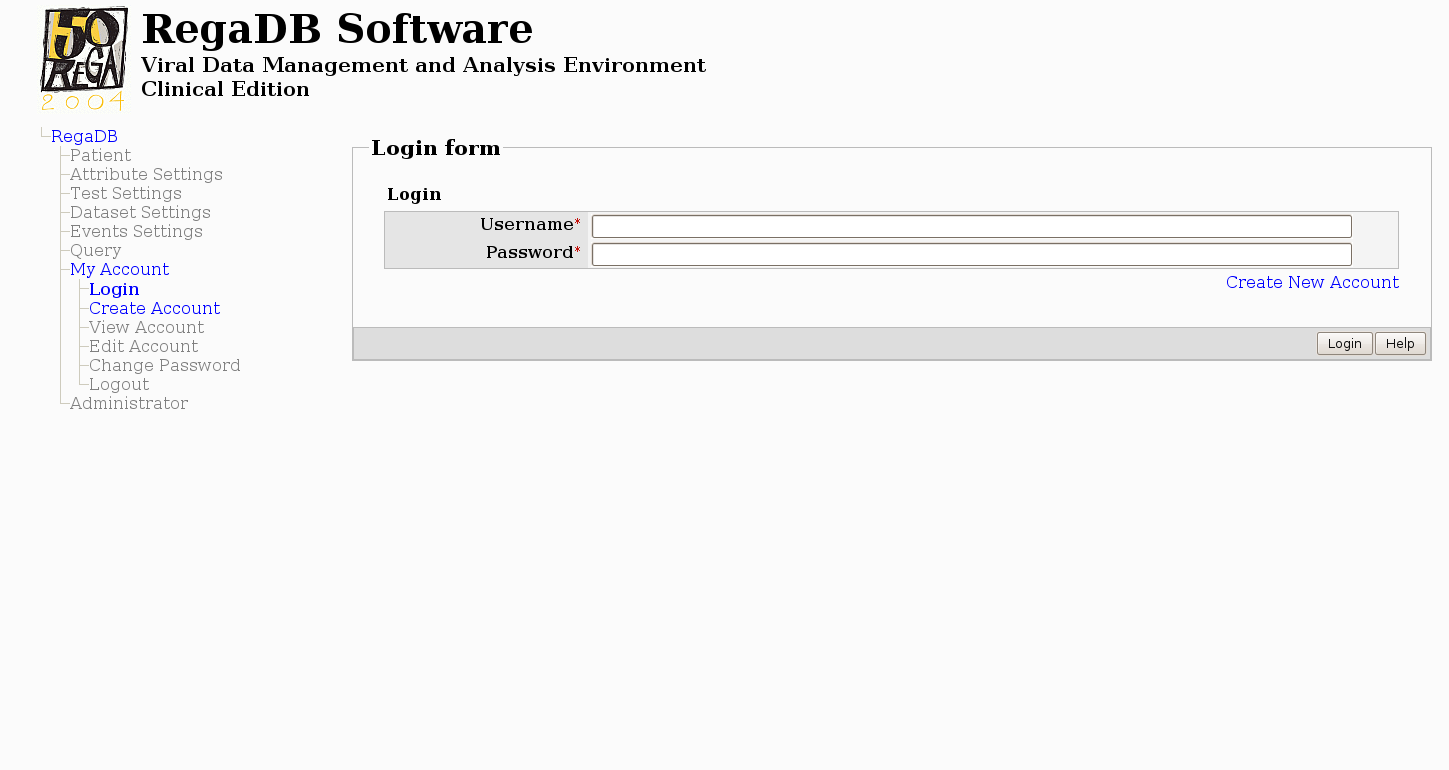
\includegraphics[width=15cm] {pics/user_config/user_1.png}}
\\
Create a new administrator by clicking on \textbf{Create new account}.
\\
\vspace{0.5cm}~ \\ \centerline{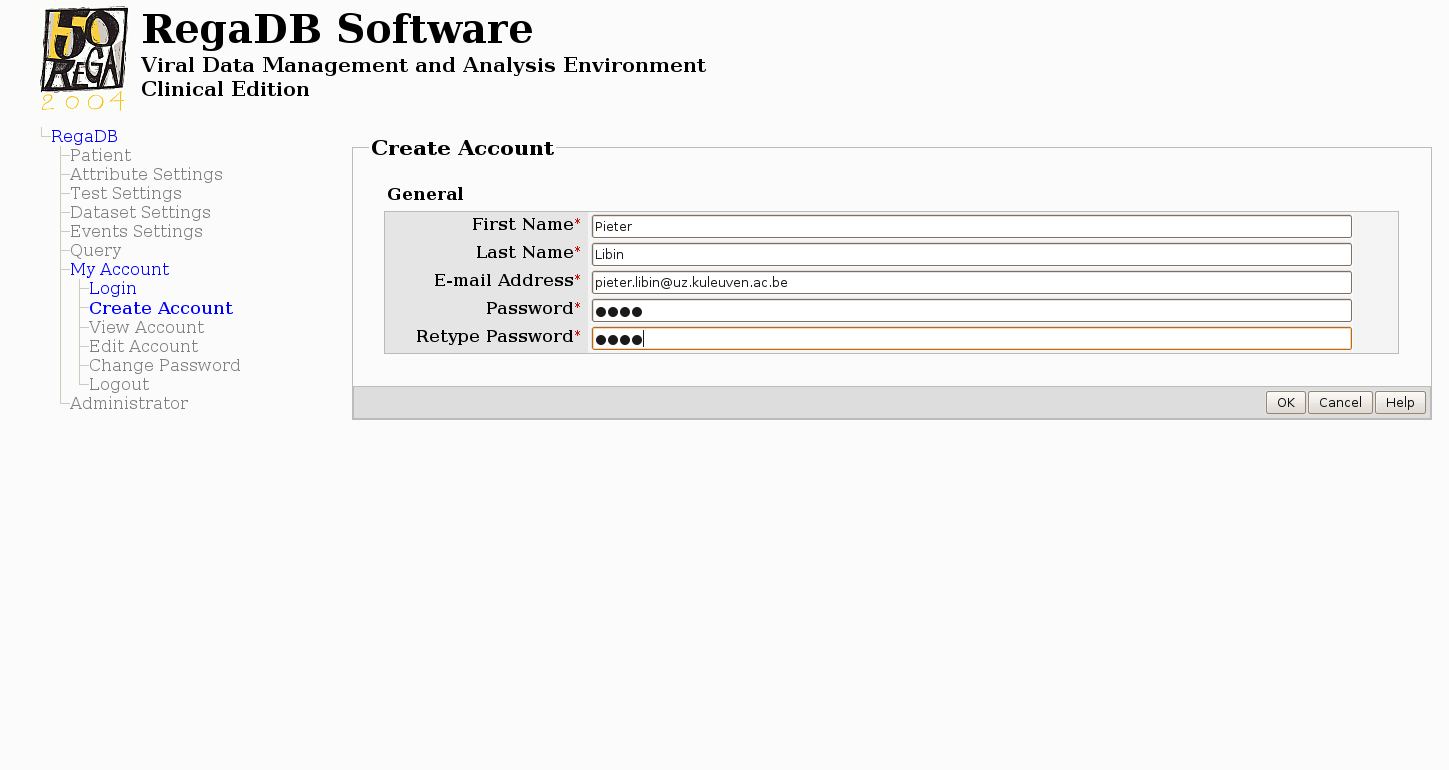
\includegraphics[width=15cm] {pics/user_config/user_2.png}}
\\
Fill in the necessary fields and click \textbf{OK}.
\\
\vspace{0.5cm}~ \\ \centerline{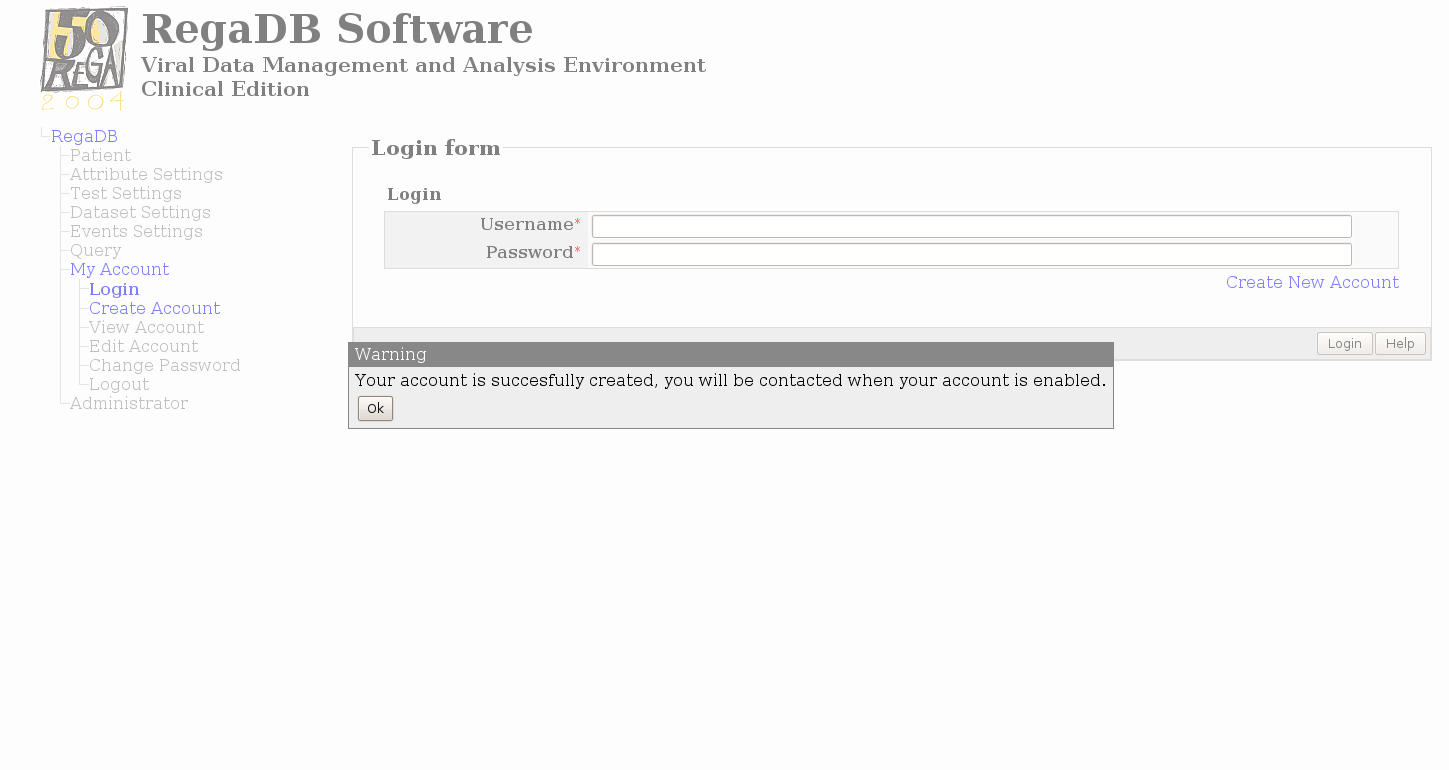
\includegraphics[width=15cm] {pics/user_config/user_3.png}}
\\
Clicking \textbf{OK} in the message box will bring you back to the login page. Now you need to activate the user by loggin in with the default user (username=admin, password=admin).
\\
\vspace{0.5cm}~ \\ \centerline{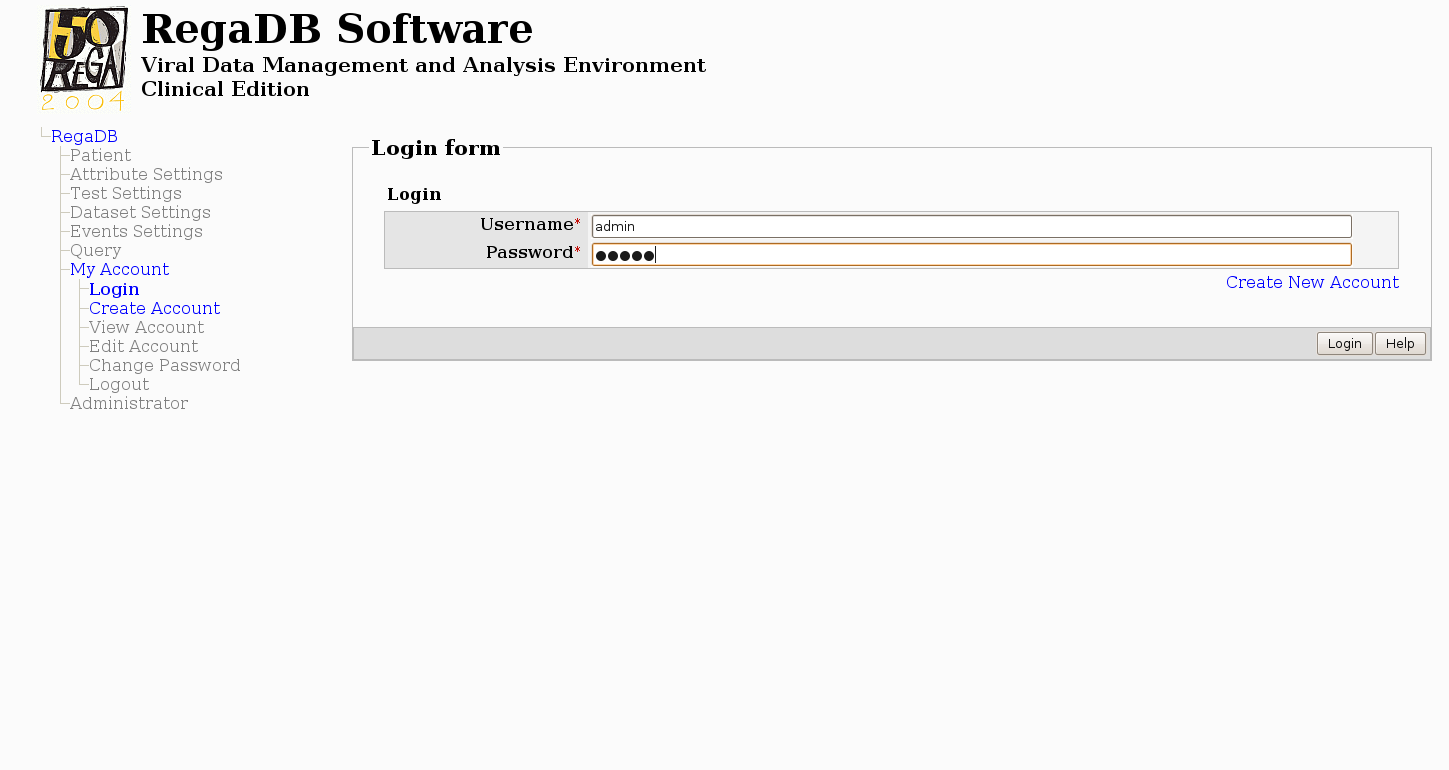
\includegraphics[width=15cm] {pics/user_config/user_4.png}}
\\
\vspace{0.5cm}~ \\ \centerline{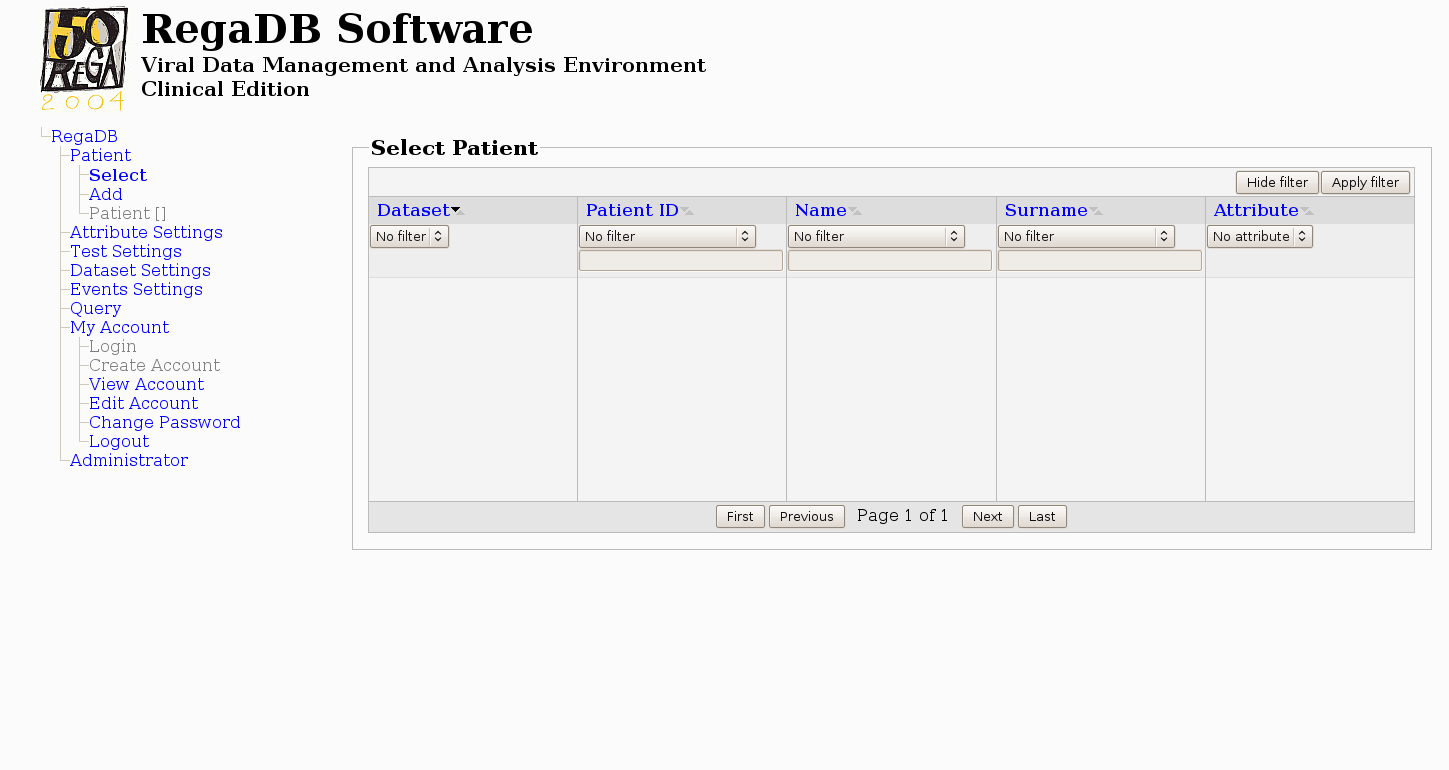
\includegraphics[width=15cm] {pics/user_config/user_5.png}}
\\
Once logged in, navigate to the Dataset menu in the navigation tree, and Add a new dataset.
\\ 
\vspace{0.5cm}~ \\ \centerline{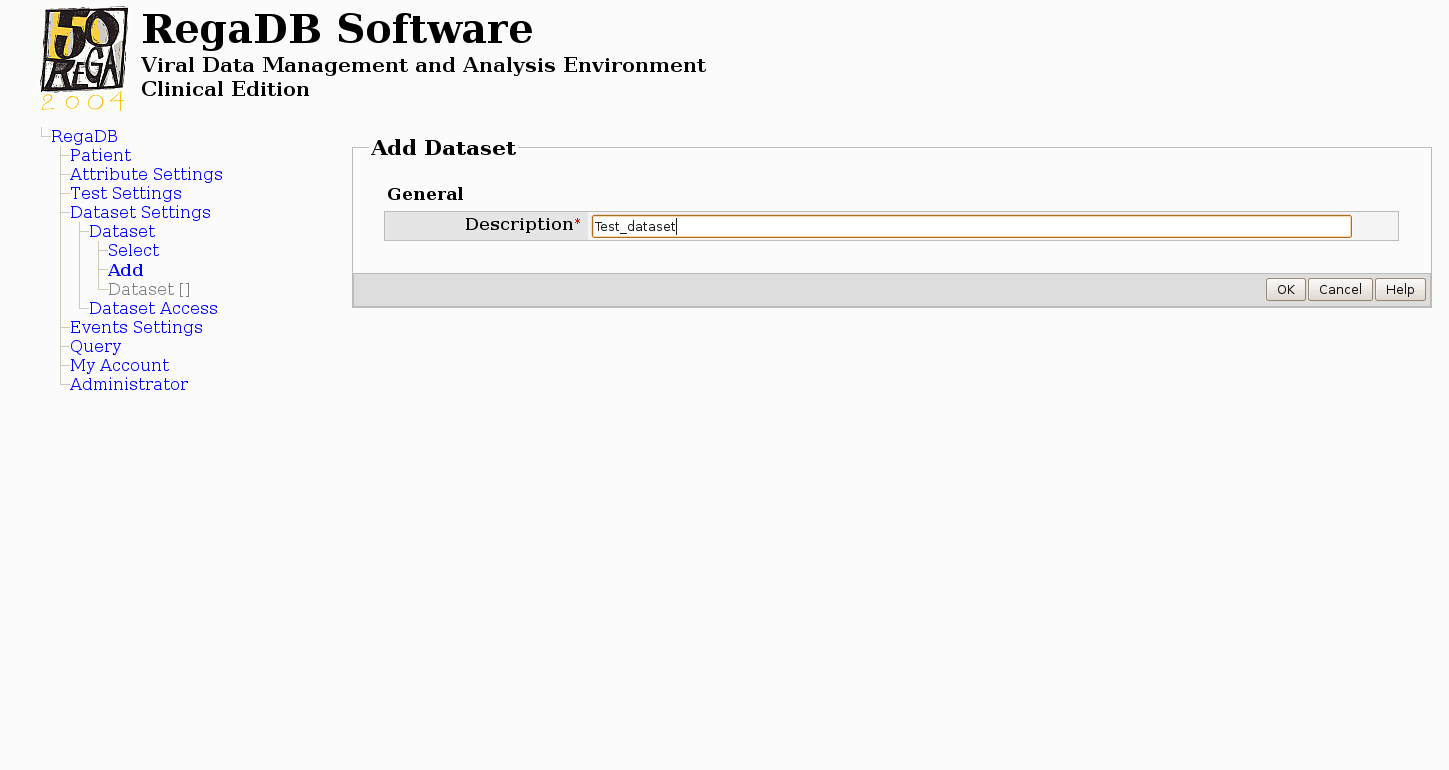
\includegraphics[width=15cm] {pics/user_config/user_7.png}}
\\
\vspace{0.5cm}~ \\ \centerline{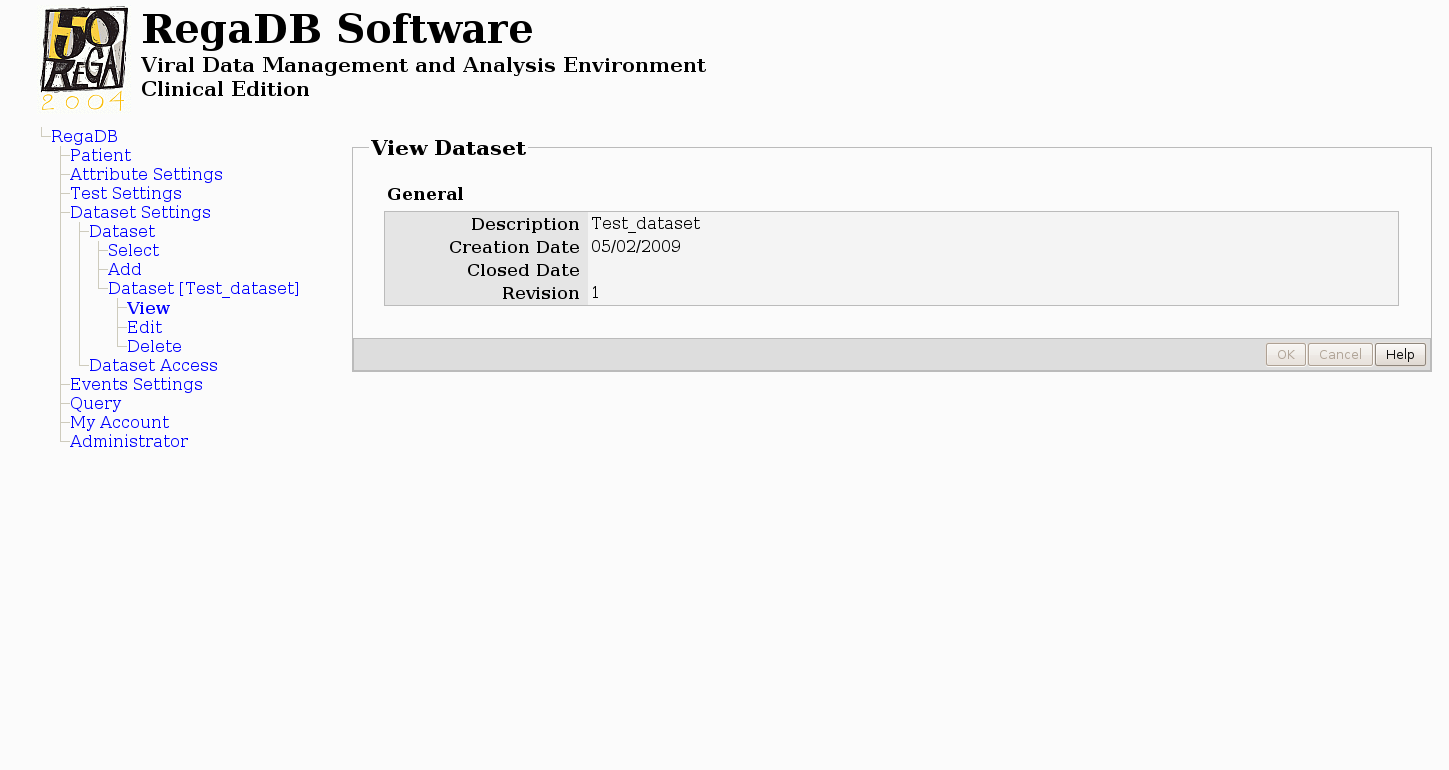
\includegraphics[width=15cm] {pics/user_config/user_8.png}}
\\
Navigate to Administrator, Not Registered Users to activate the new user.
\\
\vspace{0.5cm}~ \\ \centerline{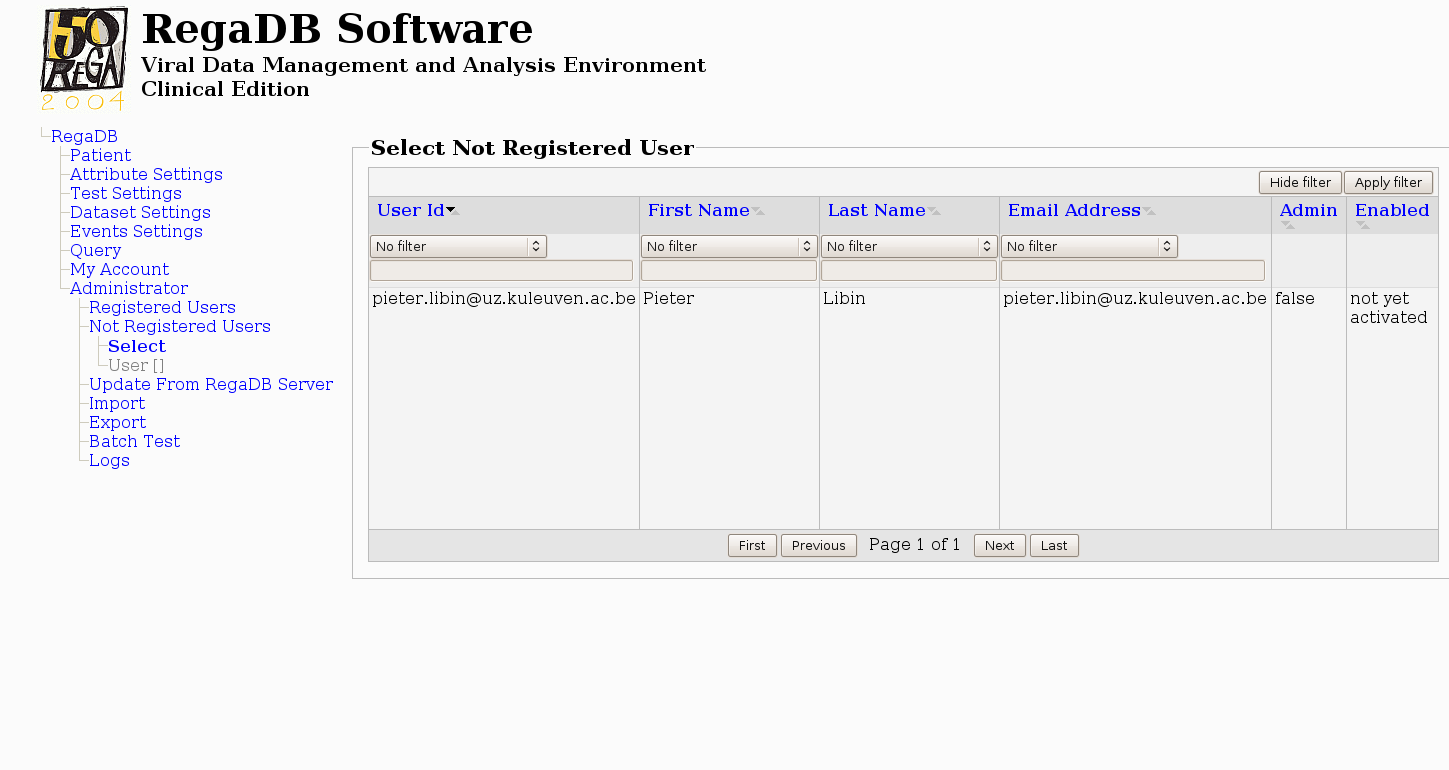
\includegraphics[width=15cm] {pics/user_config/user_9.png}}
\\
Select the newly created user.
\\
\vspace{0.5cm}~ \\ \centerline{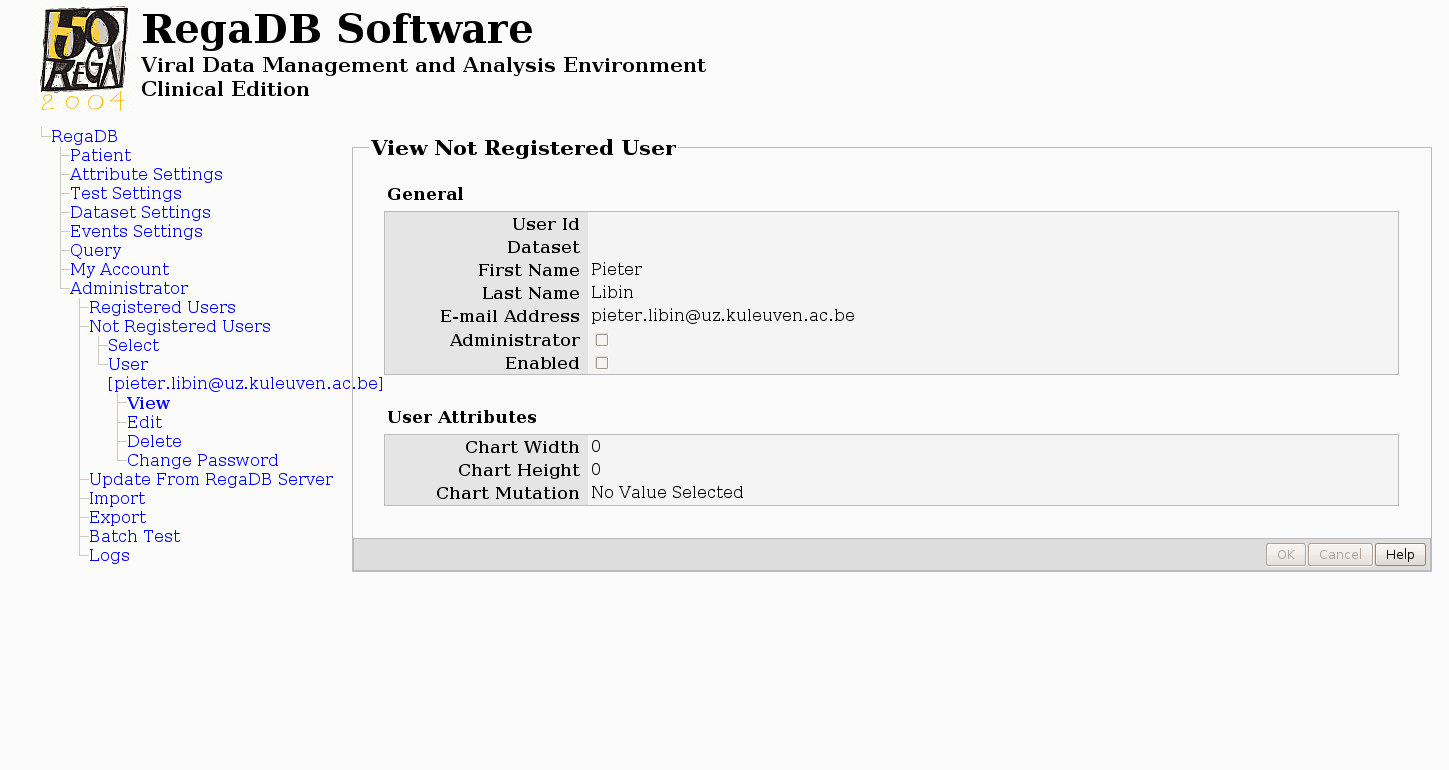
\includegraphics[width=15cm] {pics/user_config/user_10.png}}
\\
Edit this user, fill in the \textbf{User Id} and toggle on both the \textbf{Adminstrator} and \textbf{Enabled} field.
\\
\vspace{0.5cm}~ \\ \centerline{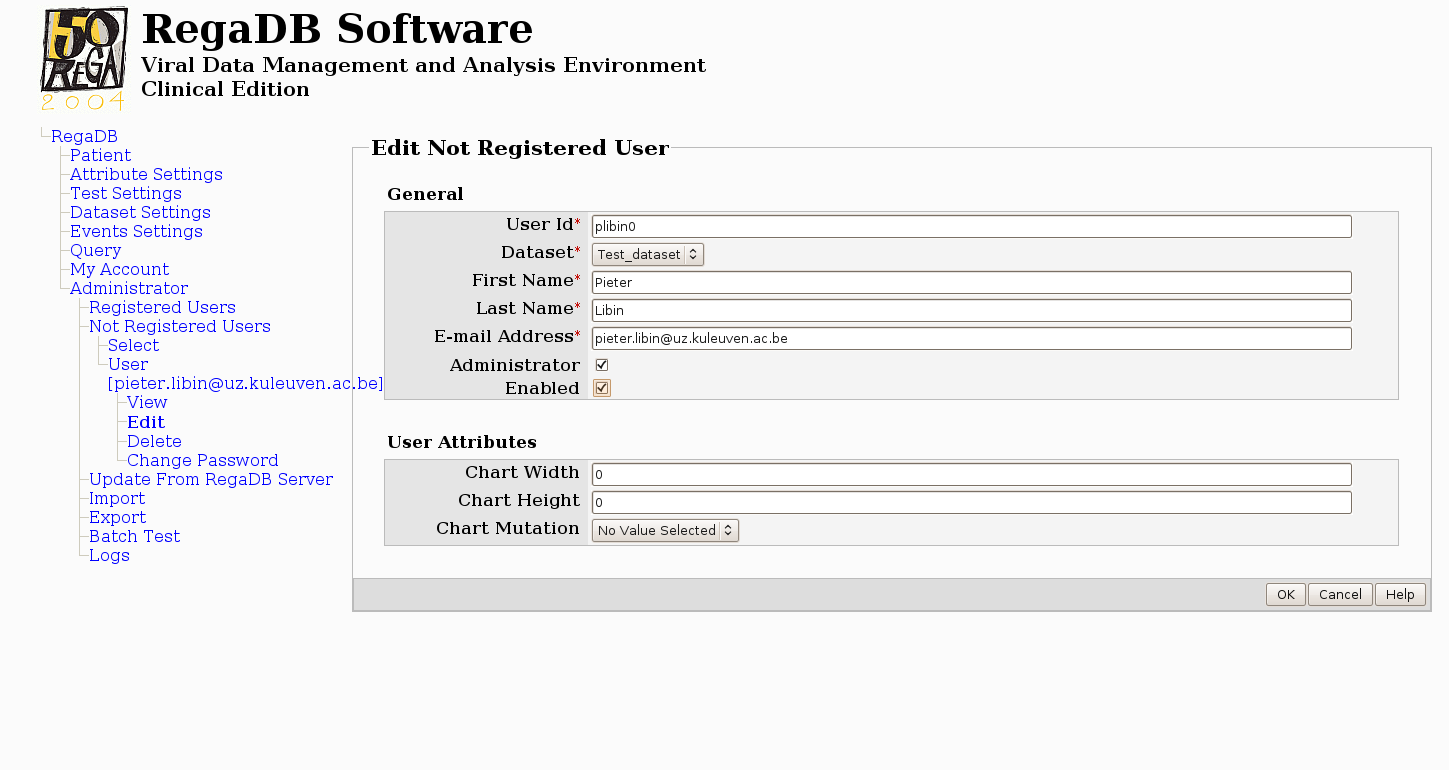
\includegraphics[width=15cm] {pics/user_config/user_11.png}}
\\
Click \textbf{OK} to confirm this action.
\\
\vspace{0.5cm}~ \\ \centerline{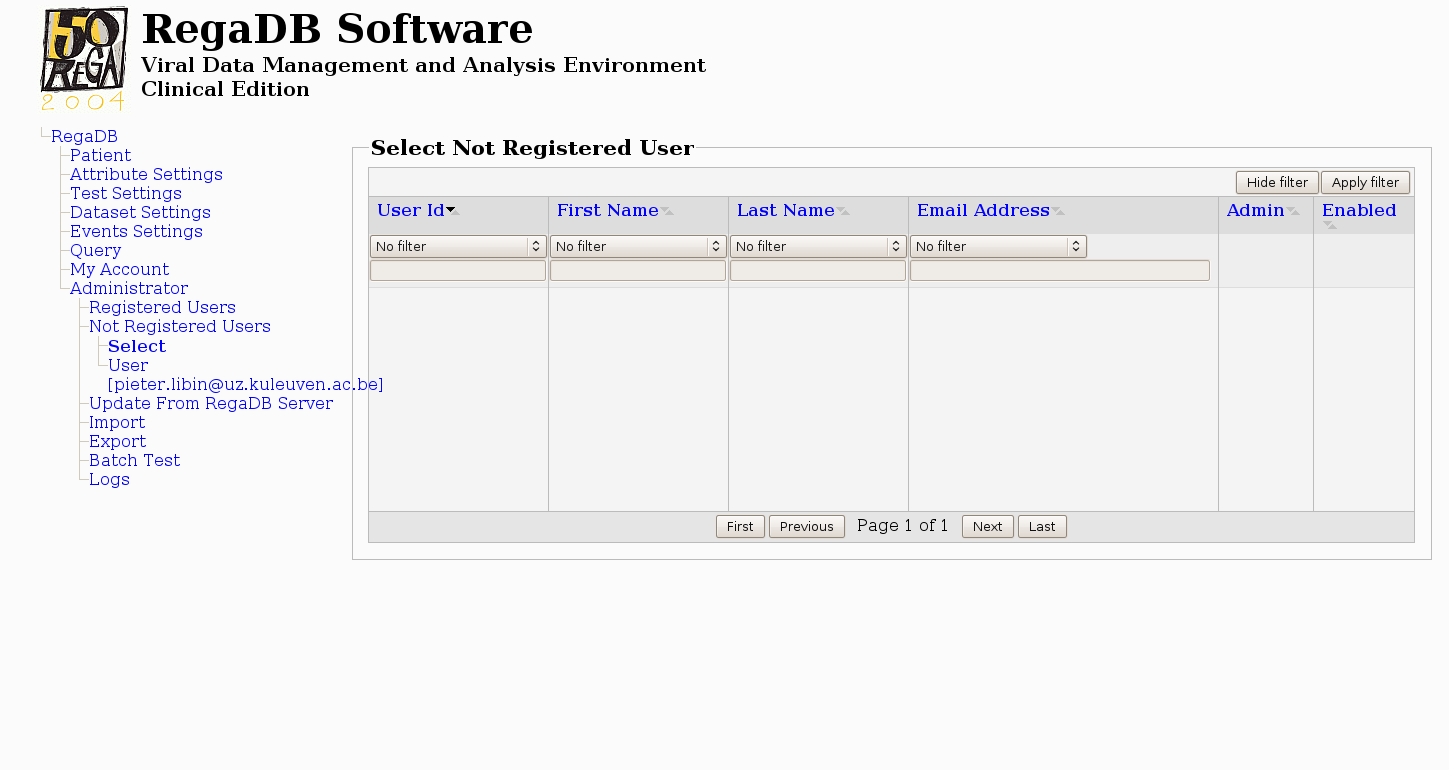
\includegraphics[width=15cm] {pics/user_config/user_12.png}}
\\
Navigate to \textbf{My Account} and log out.
\\
\vspace{0.5cm}~ \\ \centerline{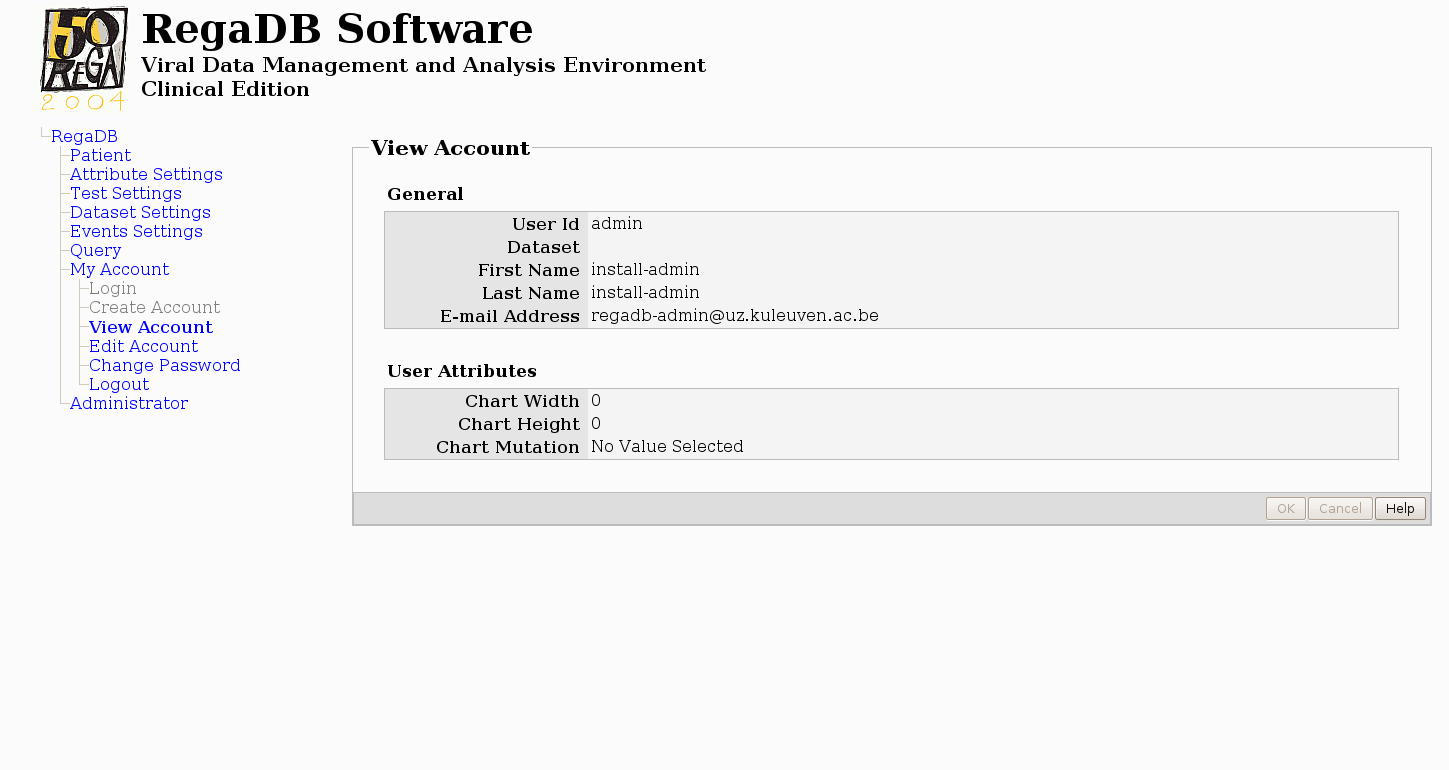
\includegraphics[width=15cm] {pics/user_config/user_13.png}}
\\
\vspace{0.5cm}~ \\ \centerline{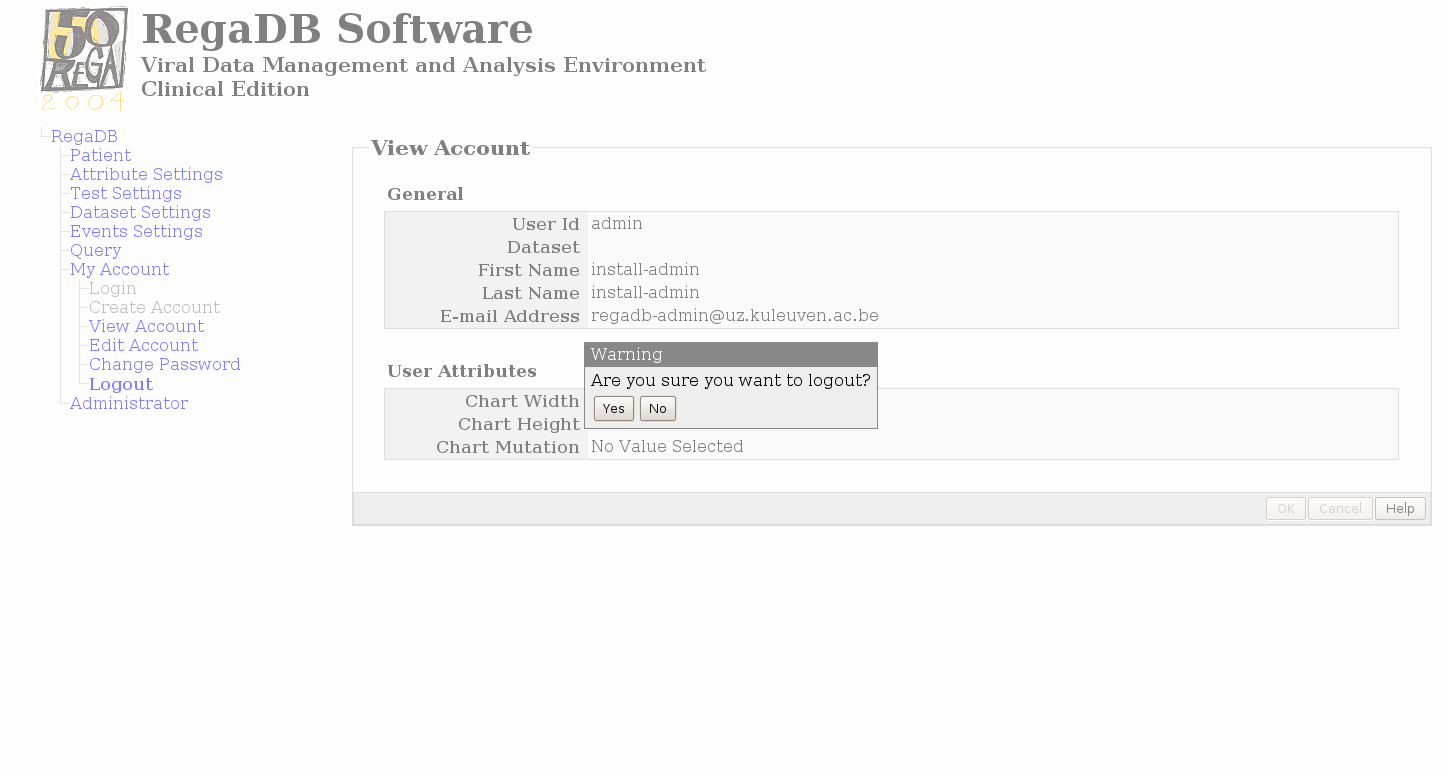
\includegraphics[width=15cm] {pics/user_config/user_14.png}}
\\
Log in as the activated user, and navigate to Administrator, Registered Users.
\\
\vspace{0.5cm}~ \\ \centerline{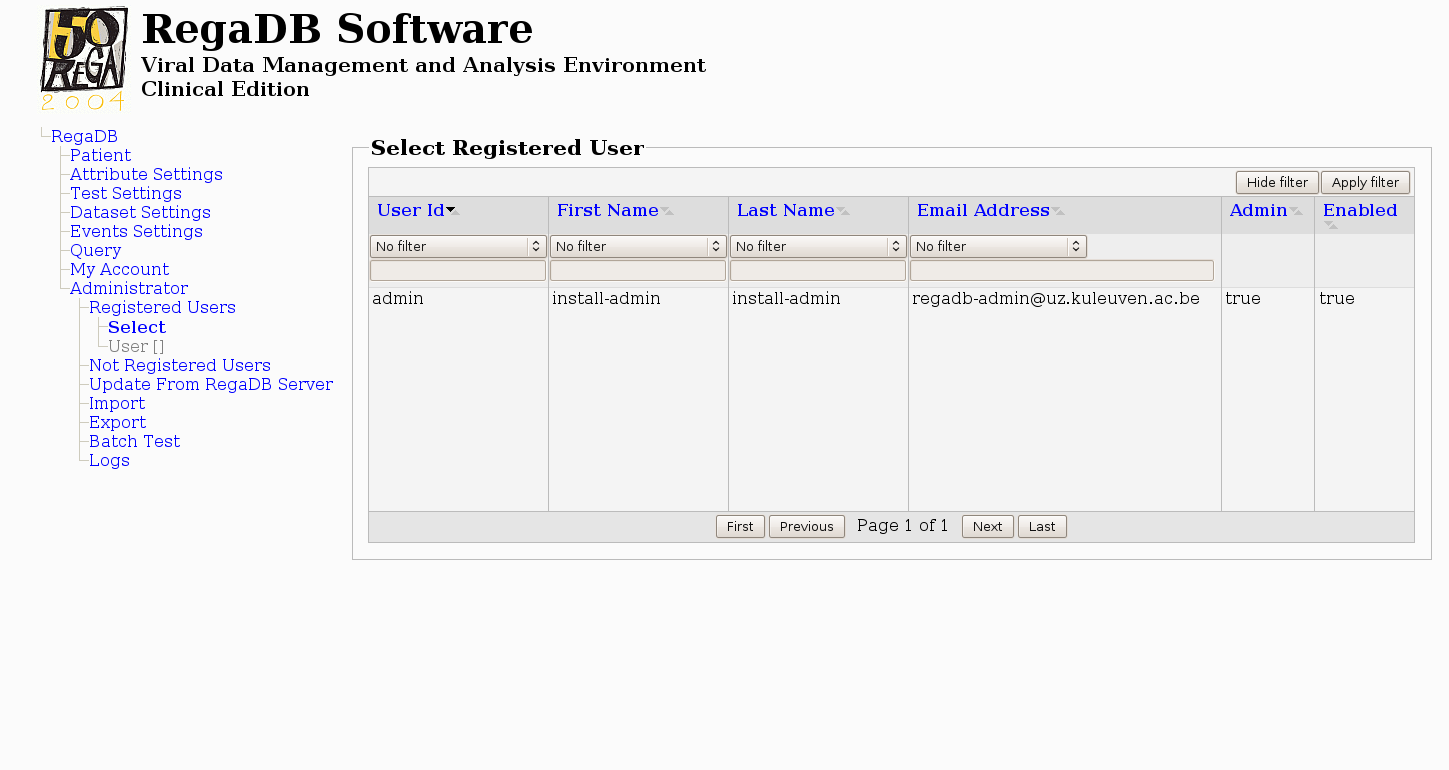
\includegraphics[width=15cm] {pics/user_config/user_15.png}}
\\
Select the default admin user.
\\
\vspace{0.5cm}~ \\ \centerline{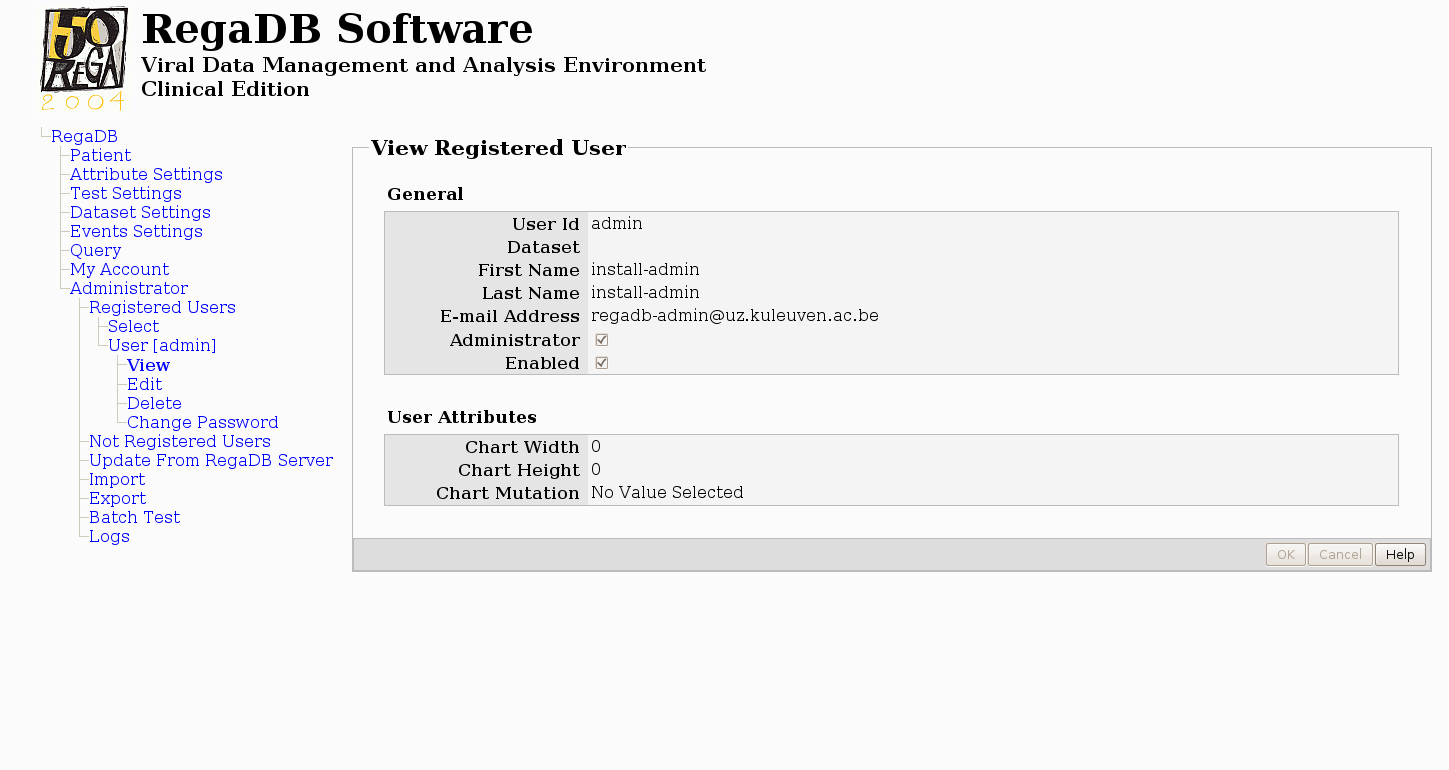
\includegraphics[width=15cm] {pics/user_config/user_16.png}}
\\
Toggle off the \textbf{Administrator} and \textbf{Enabled} fields.
\\
\vspace{0.5cm}~ \\ \centerline{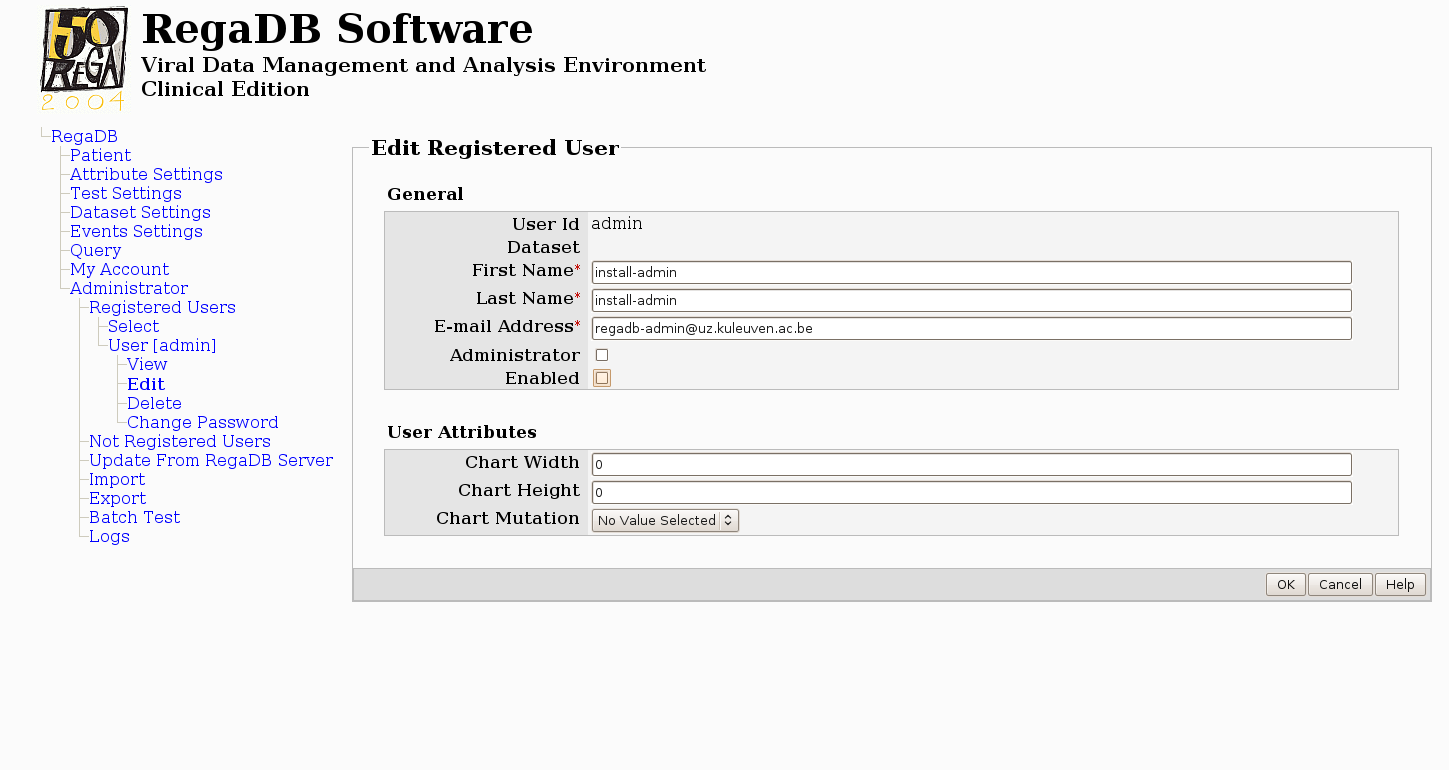
\includegraphics[width=15cm] {pics/user_config/user_17.png}}
\\
Click \textbf{OK} to confirm this action, now the default admin user will not be accessible any more.

\section{Update RegaDB with the latest auxilary data}
Navigate your browser to \textit{http://localhost:8080/regadb/RegaDB}, and login to the system.
\\
\vspace{0.5cm}~ \\ \centerline{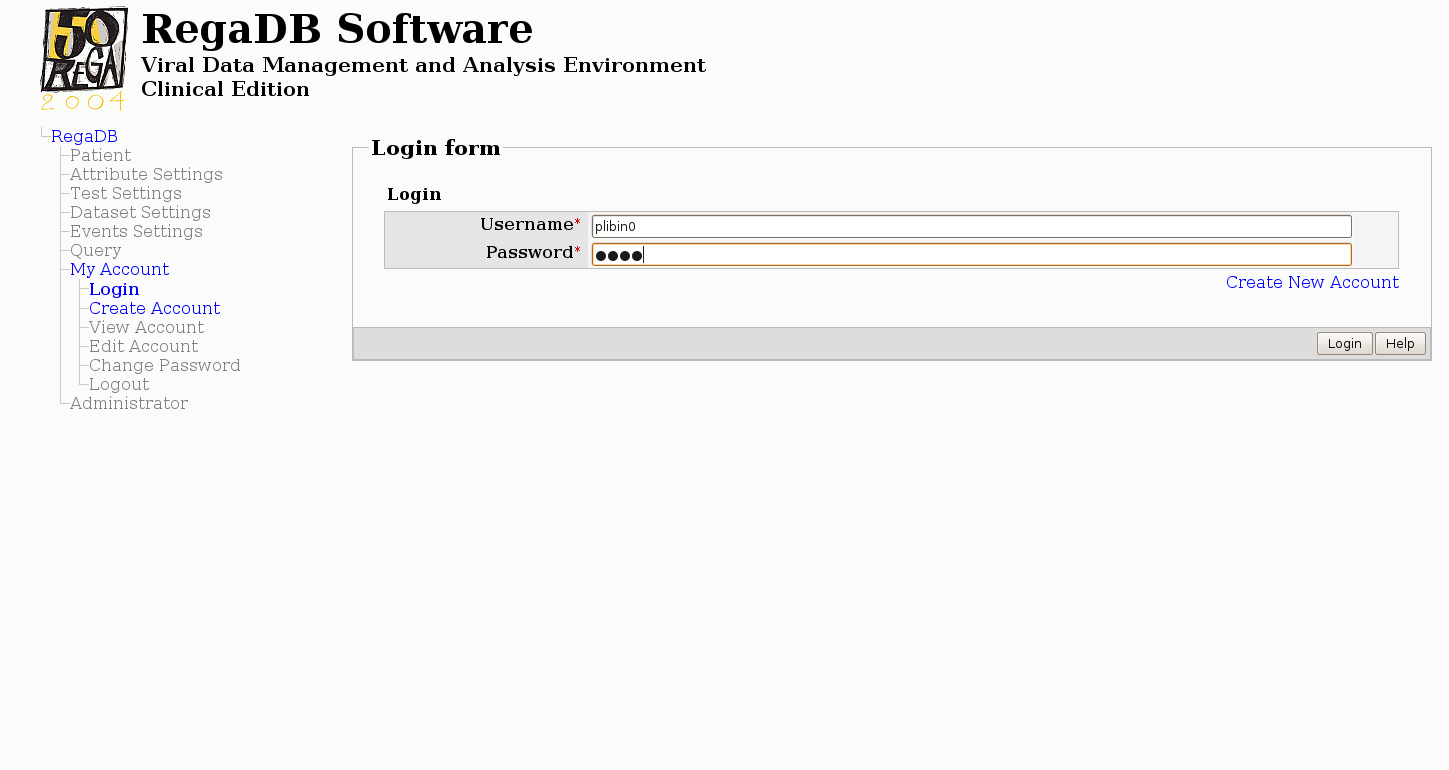
\includegraphics[width=15cm] {pics/auxilary/aux_1.png}}
\\
\vspace{0.5cm}~ \\ \centerline{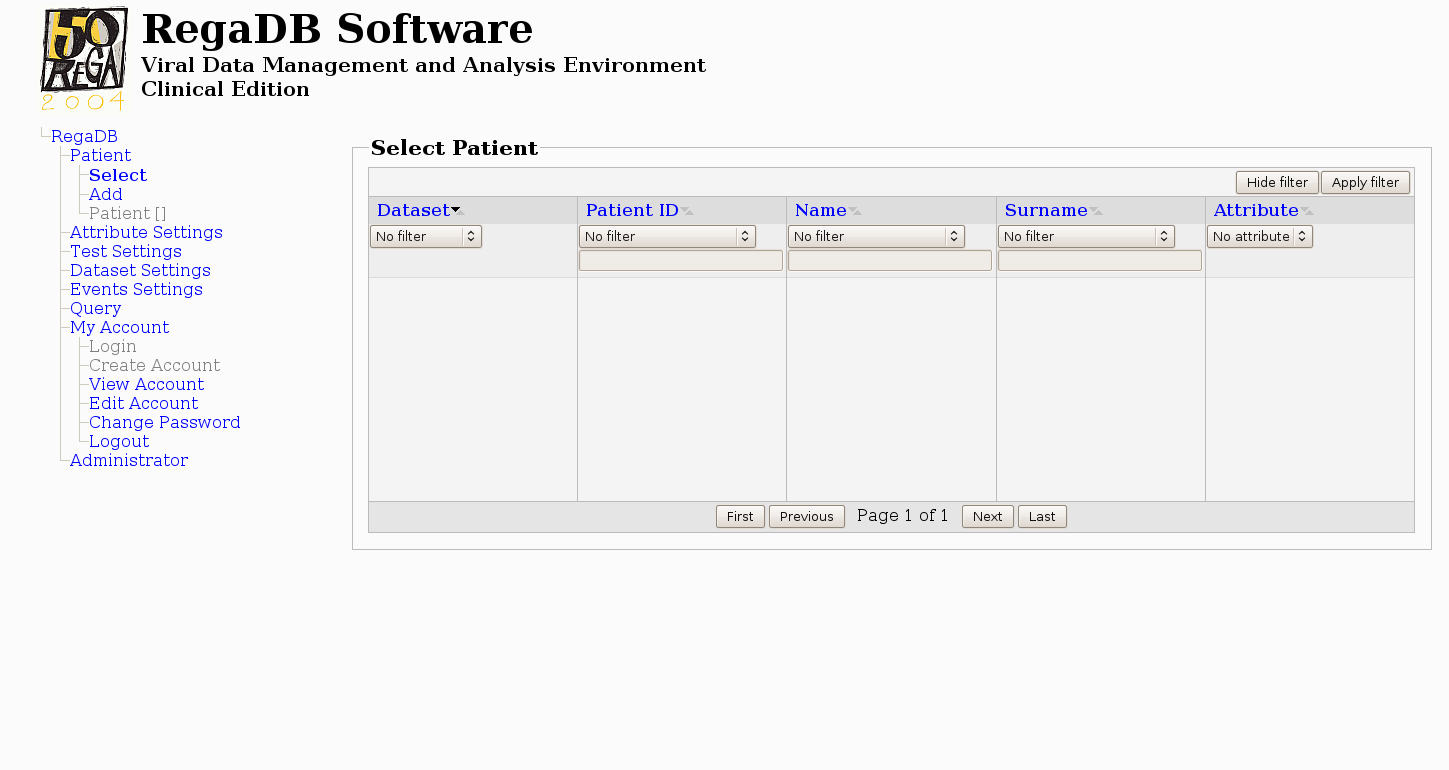
\includegraphics[width=15cm] {pics/auxilary/aux_2.png}}
\\
Navigate to the Administrator, Update from RegaDB Server page.
\\
\vspace{0.5cm}~ \\ \centerline{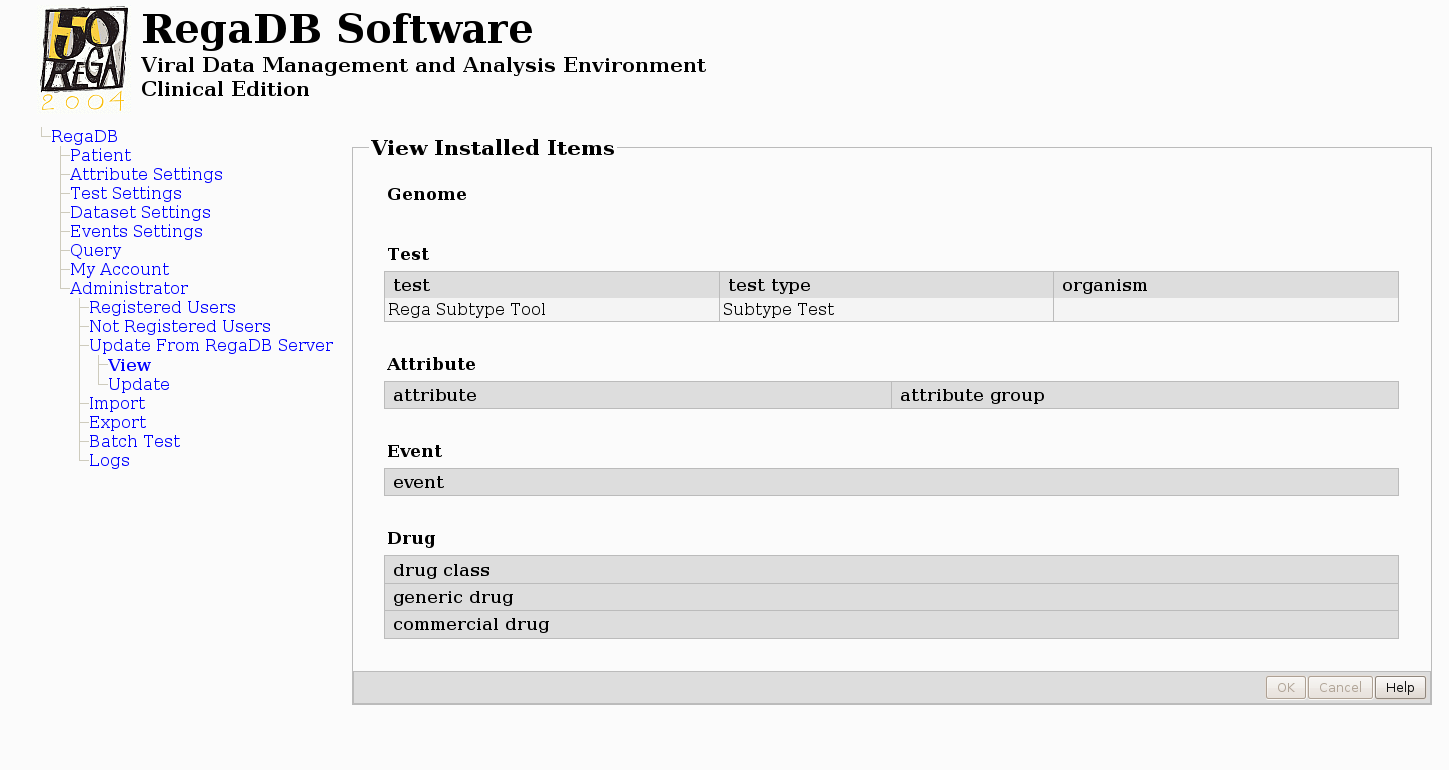
\includegraphics[width=15cm] {pics/auxilary/aux_3.png}}
\\
Click on Update, and a simulation update will be performed. This might take a few minutes, depending on your internet connection speed.
\\
\vspace{0.5cm}~ \\ \centerline{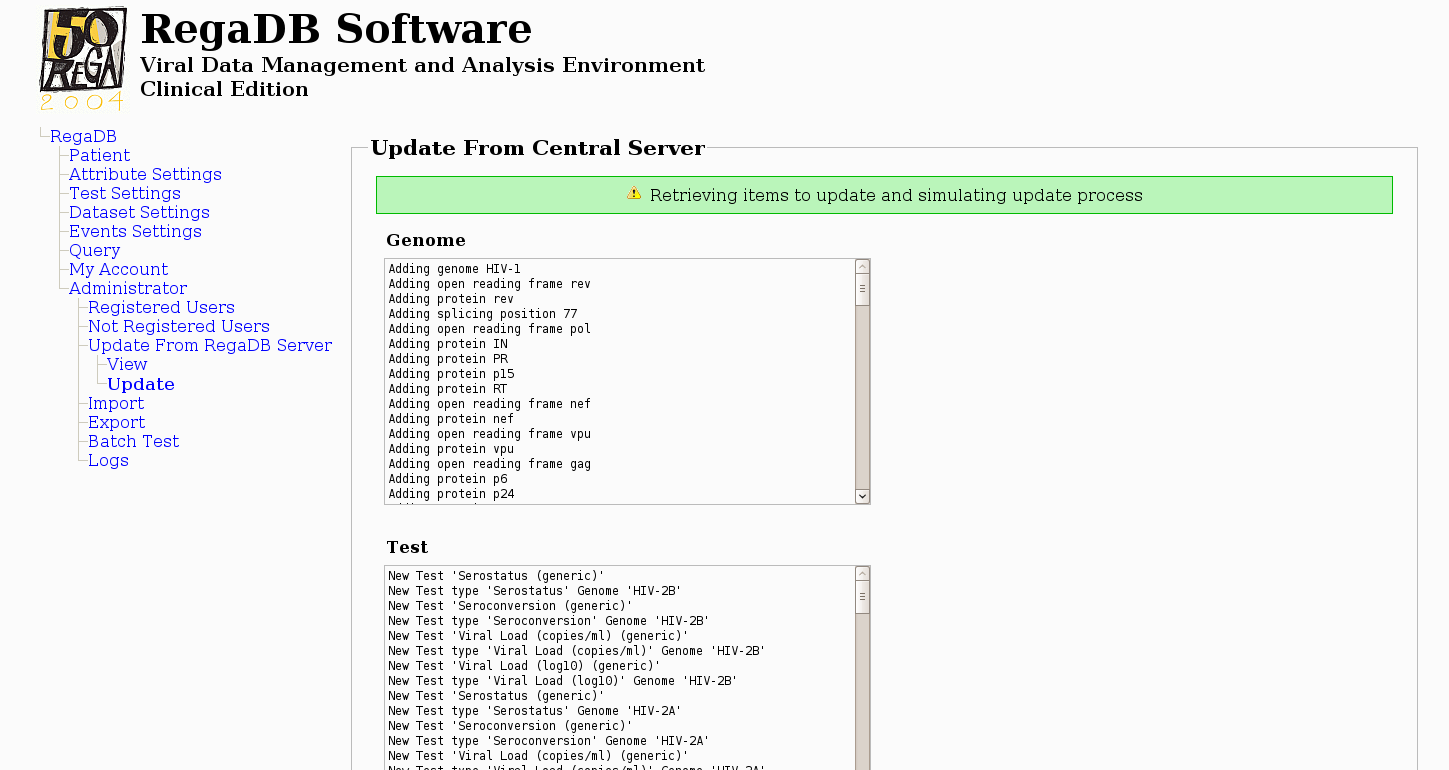
\includegraphics[width=15cm] {pics/auxilary/aux_4.png}}
\\
Click \textbf{OK} to confirm this simulation and to load the items into your local RegaDB instance. Again, this procedure might take a few minutes.
\\
\vspace{0.5cm}~ \\ \centerline{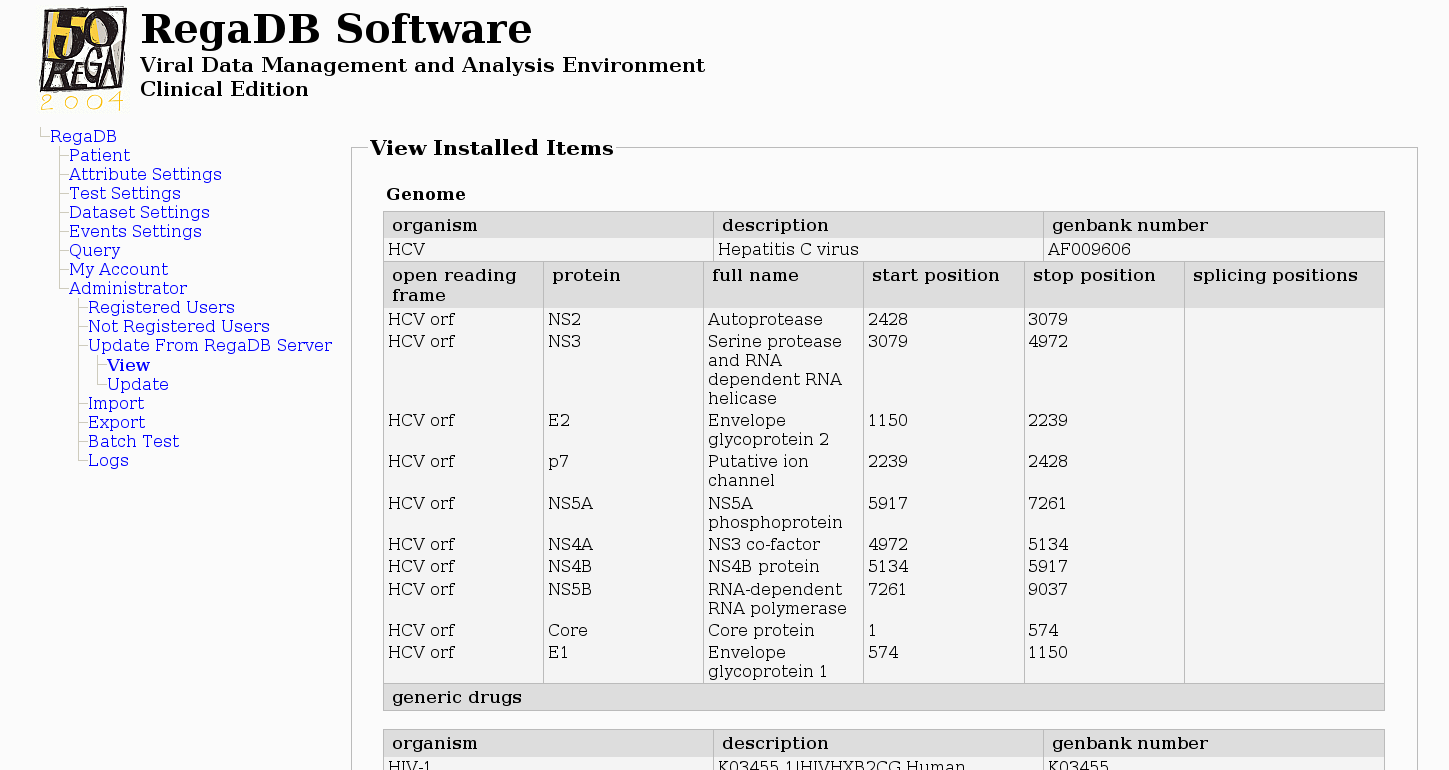
\includegraphics[width=15cm] {pics/auxilary/aux_5.png}}
\\
